\documentclass{school-22.101-notes}
\date{October 26, 2011}

\begin{document}
\maketitle

\topic{Low Energy S-Wave Approximation ($l=0$)}
\begin{figure}[ht]
    \centering
    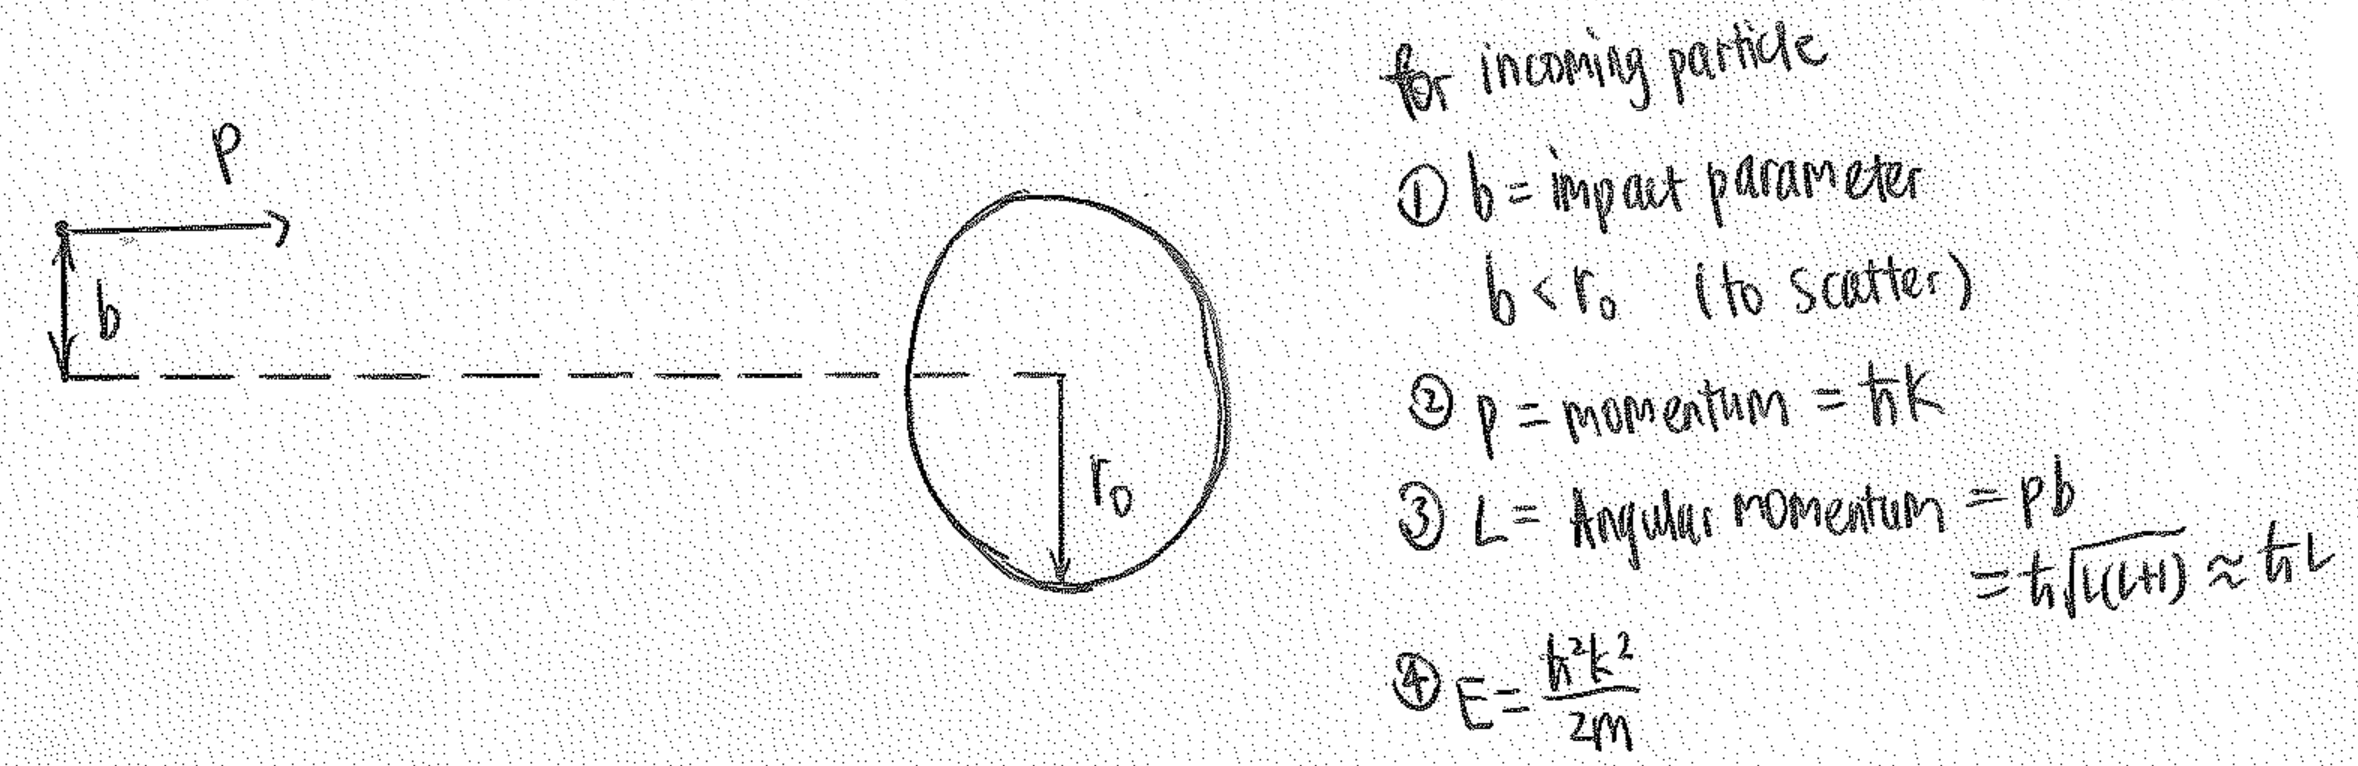
\includegraphics[width=6in]{images/scattering/np-scattering-diagram.png}
    \caption{n-p Scattering Diagram, S-Wave Approximation}
\end{figure}
\begin{enumerate}
\item A particle coming with a small incoming energy E means $k r_0 \ll 1$. This is because $E = \frac{\hbar^2 k^2}{2m} \Rightarrow k = \frac{\sqrt{2mE}}{\hbar}$, so when $E$ is small, $k$ is small. Similarly $r_0$ is reasonably small as well, hence $k r_0 \ll 1$. 

\item $ p = \hbar k$. 

\item $l=0$ because $l<kr_0 \ll 1$:
\begin{align}
L &= pb = \hbar \sqrt{l (l+1)} \approx \hbar l \Rightarrow \hbar l = pb = \hbar k b \\
\Rightarrow b &= \frac{l}{k} < r_0 \Rightarrow l < kr_0 \\
l &< k r_0 \ll 1 \Rightarrow l = 0
\end{align}

\item This is called a S-Wave Approximation. $\sigma (\theta), \sigma$ are simplified when $l=0$:
\begin{align}
\sigma (\theta) &= \frac{1}{k^2} \sin^2 \delta_0 & \sigma &= \boxed{ \frac{4 \pi}{k^2} \sin^2 \delta_0 } \label{sigma}
\end{align}

\item Observation: $\sigma$ is spherically symmetric, isotropic, because we assumed no $\theta$ dependency in S-Wave approximation. Example: when $E \approx 1 \fsp \eV \sim 10^4 \fsp \eV, \sigma = 20 \fsp b$. 

\item \textbf{Scattering Length $a$}: In the limit of low E, we define scattering length as\footnote{$a$ may be positive or negative. Here we use Krane's notation.}:
\begin{align}
\left. \begin{array}{c}
- \lim_{k\to 0} f(\theta) = a  \\
f(\theta) = \frac{1}{k} \Sum (2l+1) e^{i \delta_0} \sin \delta_0  P_l (\cos \theta) = \frac{1}{k} e^{i\theta_0} \sin \theta_0  \approx \frac{\delta_0}{k} 
\end{array} 
\right\} \Rightarrow \delta_0 = -ak
\end{align}
\begin{align}
\sigma &= 4 \pi \frac{1}{k^2} \sin^2 \delta_0 \approx 4 \pi \frac{\delta_0^2}{k^2} =  4 \pi \frac{(-ak)^2}{k^2} = 4 \pi a^2 \\
u(r) &= \frac{A_0}{k} \sin(kr + \delta_0) = \frac{a_0}{k} \sin (k(r-a)) \xrightarrow{\mathrm{small \fsp k}} \frac{a_0}{k} (k(r-a))
\end{align} 
The above expression suggests that $a$ behaves like an intercept.

\begin{figure}
    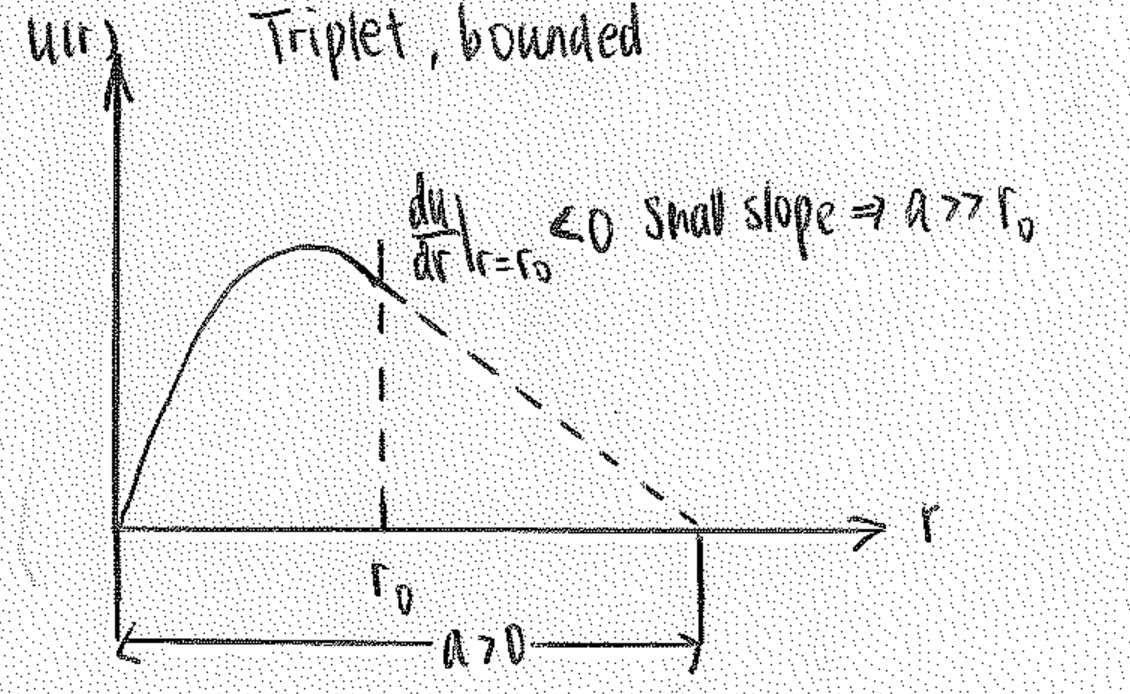
\includegraphics[width=3in]{images/scattering/s-wave-triplet.png}
    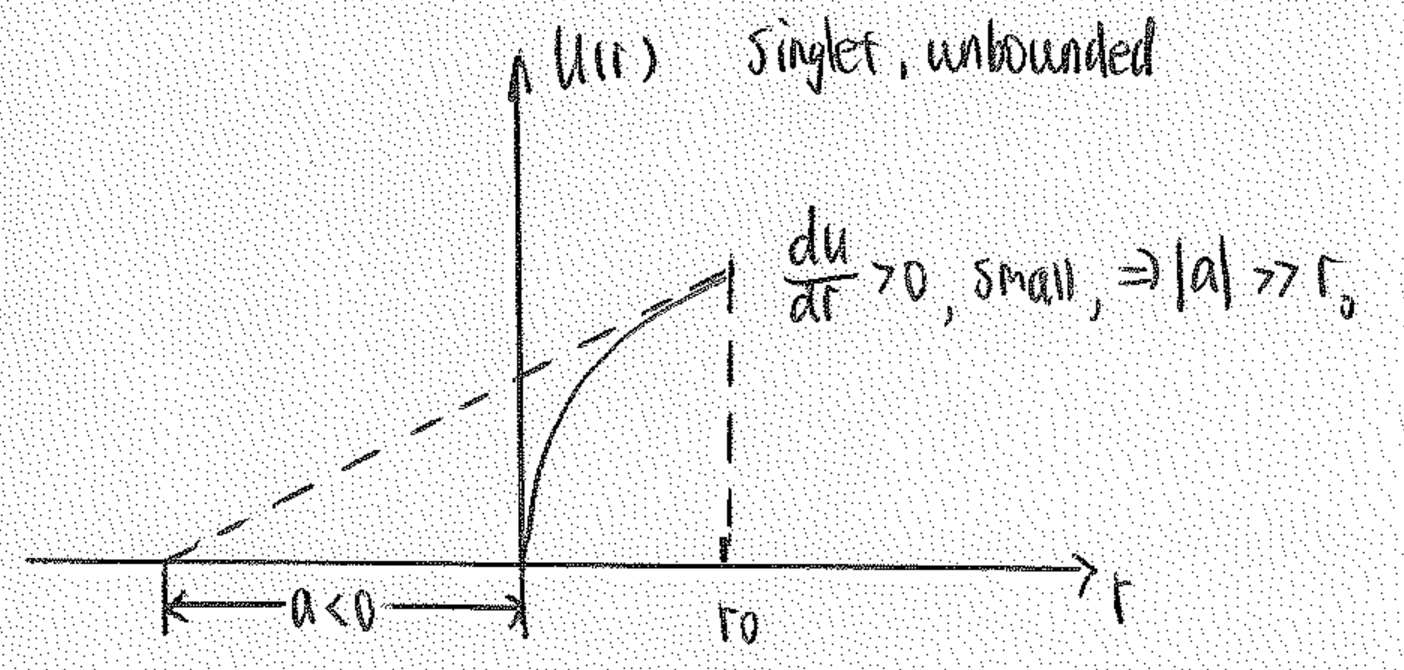
\includegraphics[width=3in]{images/scattering/s-wave-singlet.png}    
    \caption{Singlet vs. Triplet Configuration for Low Energy ($E<10 \fsp \mathrm{keV}$)\label{scattering-s-wave}}
\end{figure}
Implications of Figure~\ref{scattering-s-wave}:
\begin{itemize}
\item Sign of $a$:  positive $a$ refers to triplet/bound state, negative $a$ refers to singlet/unbounded state. 
\item $a \gg r_0$. 
\item $a$ is `scattering amplitude' because 
\eqn{ \psi_{\mathrm{sc}} = f_0 \frac{e^{ikr}}{r} = \frac{\delta_0}{k} \frac{e^{ikr}}{r} = -a \frac{e^{ikr}}{r}  }
\end{itemize}
\end{enumerate}



\end{document}
